\section{Analysis of Features 1 and 2}

\subsection*{Empirical Results}

To evaluate the discriminative power of the first two features, we analyze their class-conditional means, variances, 1D histograms, and 2D scatter plots. 

\textbf{Distributions and Overlap:} 
Based on the histograms (\texttt{feature\_1\_histogram.png} and \texttt{feature\_2\_histogram.png}), the distributions for both the "Genuine" (label 1) and "Fake" (label 0) classes are strictly unimodal, exhibiting a single, distinct peak. However, the classes exhibit a massive, nearly total overlap. As seen in the scatter plot (\texttt{features\_1\_2\_scatter.jpg}), both distributions are perfectly centered at the origin $(0,0)$, creating a dense intersecting cluster.

\textbf{Statistical Metrics:}
The computed statistics perfectly reflect this visual overlap:
\begin{itemize}
    \item \textbf{Means:} The means are virtually identical and centered near zero. For Feature 1, the Fake mean is $0.0029$ and Genuine is $0.0005$. For Feature 2, the Fake mean is $0.0187$ and Genuine is $-0.0085$.
    \item \textbf{Variances:} While the means are identical, the variances are heavily inverted between the axes. For Feature 1, the Genuine class has a massive variance ($1.4302$) compared to Fake ($0.5696$). Conversely, for Feature 2, the Fake class has the dominant variance ($1.4209$) compared to Genuine ($0.5783$).
\end{itemize}

\begin{figure}[H]
    \centering
    \begin{minipage}{0.48\textwidth}
        \centering
        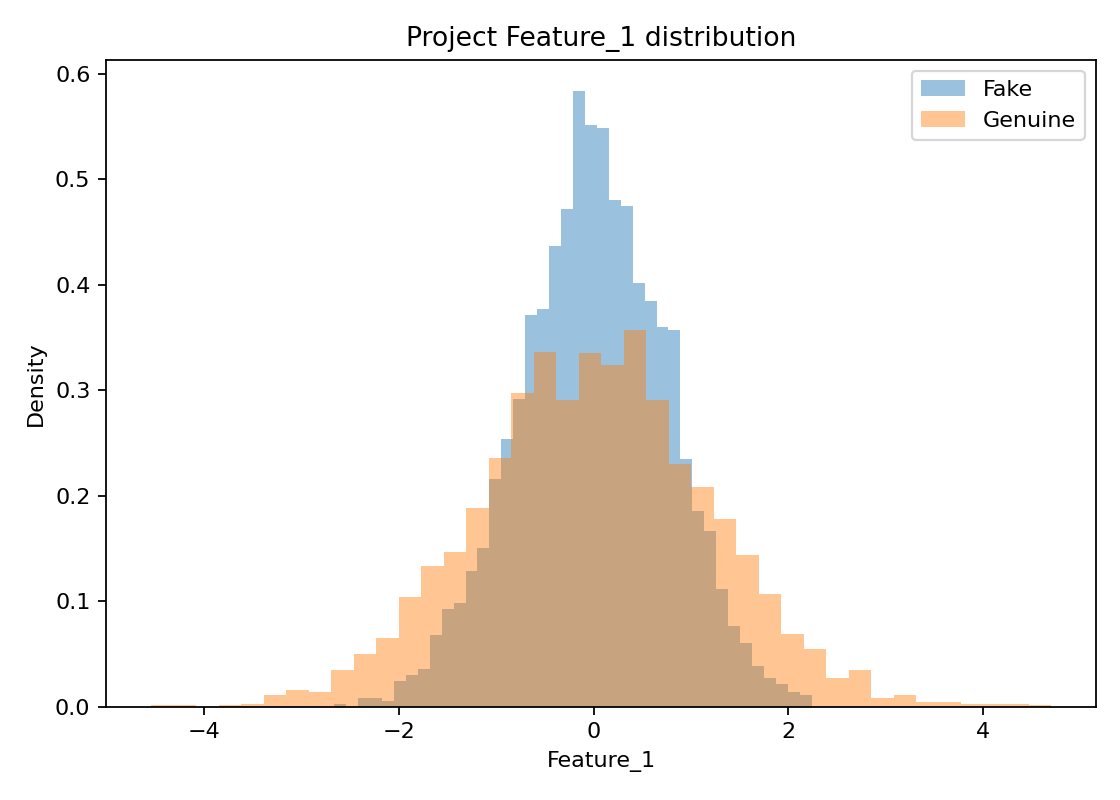
\includegraphics[width=\linewidth]{histograms/feature_1_histogram.png}
        \caption{Histogram of Feature 1.}
    \end{minipage}\hfill
    \begin{minipage}{0.48\textwidth}
        \centering
        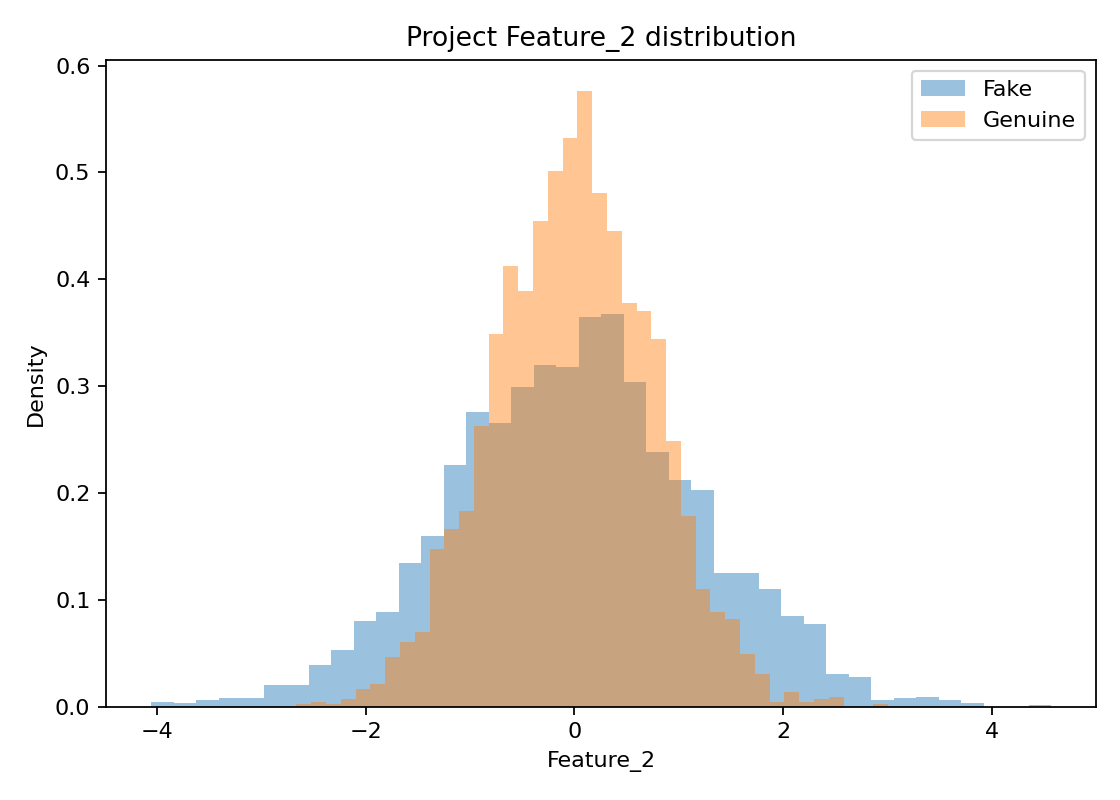
\includegraphics[width=\linewidth]{histograms/feature_2_histogram.png}
        \caption{Histogram of Feature 2.}
    \end{minipage}
\end{figure}

\begin{figure}[H]
    \centering
    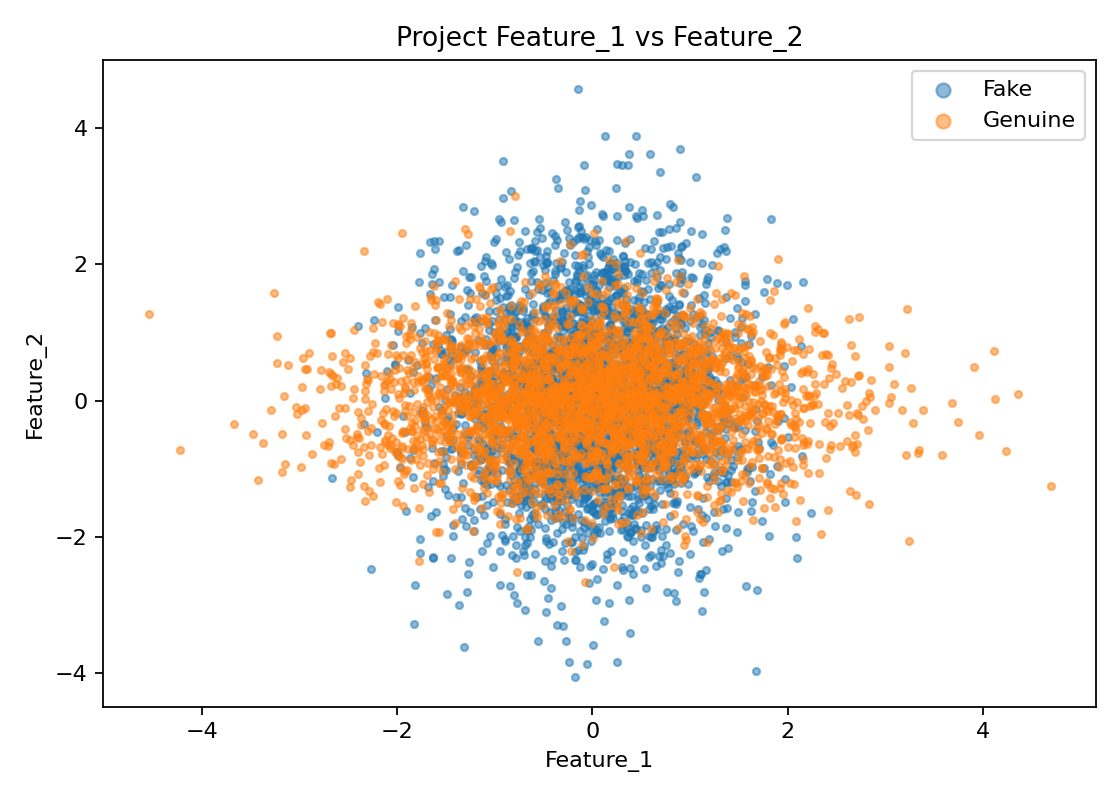
\includegraphics[width=0.6\textwidth]{scatters/features_1_2_scatter.png}
    \caption{Scatter plot of Feature 1 vs Feature 2, illustrating the inverted variance "cross" topology.}
    \label{fig:scatter_1_2}
\end{figure}

\subsection*{Theoretical Analysis}

The statistical inversion of the variances combined with identical means yields a highly specific geometric topology. Because the centers of mass for both classes sit exactly on top of each other at $(0,0)$, there is no spatial shift between them. Instead, the classes differentiate themselves purely by their spread.

The Fake class spreads vertically along the Feature 2 axis, while the Genuine class spreads horizontally along the Feature 1 axis. In a 2D space, this creates a distinct "cross" or "plus-sign" intersection (clearly visible in Figure \ref{fig:scatter_1_2}). 

\subsection*{Motivation and Future Insights}

This specific feature geometry provides critical insight that directly predicts the performance of our classifiers in subsequent laboratories (Lab 6 and Lab 10):

\begin{enumerate}
    \item \textbf{Failure of Linear Models:} Because the centroids are identical, a globally linear decision boundary (like standard Logistic Regression) cannot effectively separate these classes. A straight line drawn through the origin will inevitably misclassify half of the cross.
    \item \textbf{Catastrophic Failure of Tied MVG:} This topology perfectly explains why the Tied Covariance MVG performed so poorly throughout the project. The Tied MVG forces both classes to share a single, averaged covariance matrix. By averaging the horizontal Genuine spread and the vertical Fake spread, the Tied MVG assumes both classes are identical, symmetric circles. It completely destroys the only discriminative geometric information available in these features.
    \item \textbf{Success of Quadratic/Non-Linear Models:} To separate a cross-shaped distribution, a classifier must be able to draw an ellipse or a closed geometric boundary. This theoretically justifies why models capable of generating quadratic boundaries (like the Standard MVG) or highly localized non-linear boundaries (like the RBF Kernel SVM used in our final fusion) vastly outperformed the linear baselines.
\end{enumerate}